\chapter{METODOLOGI PENELITIAN}
\section{Studi Literatur}
Studi literature dilakukan dengan mempelajari penelitian yang berkaitan dengan materi \emph{hand gesture recognition}, \emph{Retinex} dan \emph{Convolutional Neural Network} yang  diperoleh dari berbagai sumber seperti buku, artikel, jurnal dan sumber lain yang diperoleh dari internet.
\section{Alat dan Bahan}
\subsection{Alat}
\begin{enumerate}
\item PC/Laptop dengan spesifikasi processor Intel (R) Core i5-8300H CPU @2,4 GHz, GPU NVIDIA 1050, RAM 8 GB, sistem operasi Linux 64 bit.
\item Webcam Logitech C270
\item Dimmer
\item Kain	
\item Lux Meter
\end{enumerate}
\subsection{Bahan}
\begin{enumerate}
	\item Dataset gestur tangan 
\end{enumerate}
\section{Prosedur Kerja}
\subsection{Analisis dan Perancangan Sistem}
Alur penelitian yang akan dilakukan dalam penelitian ini memiliki beberapa tahapan diantaranya pengambilan dataset gestur, training data dan tahap paling akhir adalah pengujian. Alur kegiatan penelitian yang akan dilakukan secara garis besar ditunjukan pada Gambar 4.1.
% TODO: \usepackage{graphicx} required
\begin{figure}[H]
	\centering
	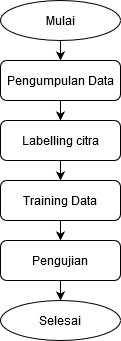
\includegraphics[width=0.2\linewidth]{Rencana}
	\caption{Alur Kegiatan Penelitian}
	\label{fig:screenshot006}
\end{figure}
Rancangan pengujian sistem ditunjukan pada Gambar 4.2 yang dimulai dengan \emph{input} dari webcam secara \emph{realtime} sehingga setiap frame akan di proses nantinya.
Setiap frame dengan citra RGB akan dilewatkan pada algoritme \emph{Retinex} untuk dilakukan perbaikan kualitas citra dengan harapan meningkatkan kontras pada sebuah citra.
% TODO: \usepackage{graphicx} required
\begin{figure}[H]
	\centering
	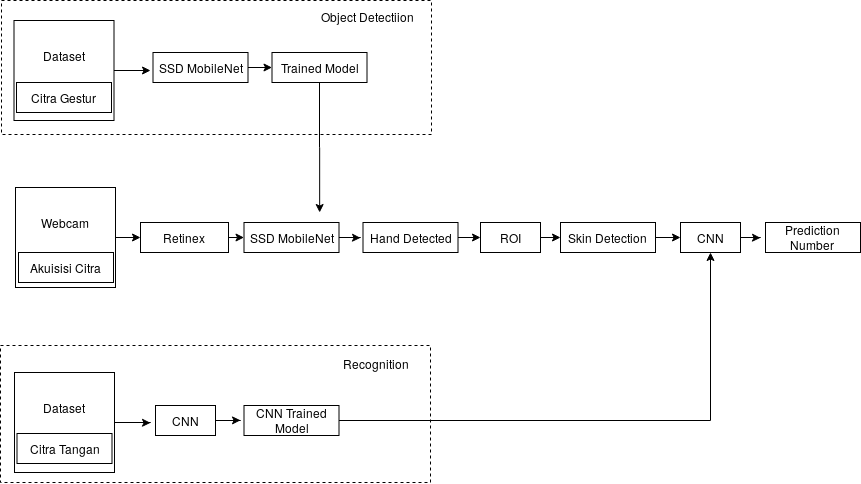
\includegraphics[width=0.9\linewidth]{rancangan}
	\caption{Rancangan Pengujian Sistem}
	\label{fig:rancangan}
\end{figure}
\noindent Setelah citra mengalami peningkatan kontras kemudian sistem akan melakukan deteksi tangan dengan \emph{SSD MobileNet} yang kemudian citra tangan tersebut akan diambil sebagai ROI. 
Citra hasil ROI akan dilakukan segmentasi menggunakan \emph{skin detection}. Hasil segmentasi akan diklasifikasikan dengan model CNN yang telah di training sebelumnya.
Keluaran dari sistem ini akan menampilkan klasifikasi angka yang terdeteksi.
\section{Pengumpulan Data}
Data pelatihan dibagi menjadi dua, yaitu dataset citra gestur tangan yang mengacu pada ASL dan dataset citra tangan biasa untuk \emph{object detection}.
Kedua dataset ini merupakan dua hal yang berbeda tujuan. 
Dataset ASL digunakan untuk proses pengenalan gestur dan dataset \emph{object detection} digunakan untuk mendeteksi adanya tangan atau tidak.

Dataset gestur tangan ASL menggunakan dataset public dari \emph{Massey University}. Dataset tersebut berisi 2425 citra yang dibagai dalam 36 kelas, yaitu 26 untuk huruf A-Z dan 10 kelas untuk angka 0-9. Pengambilan dataset dilakukan oleh 5 individu dengan variasi cahaya yang berbeda. Contoh dataset \emph{Massey University} dapat dilihat pada Gambar 4.3 (Barczak et al., 2011).
% TODO: \usepackage{graphicx} required
\begin{figure}[H]
	\centering
	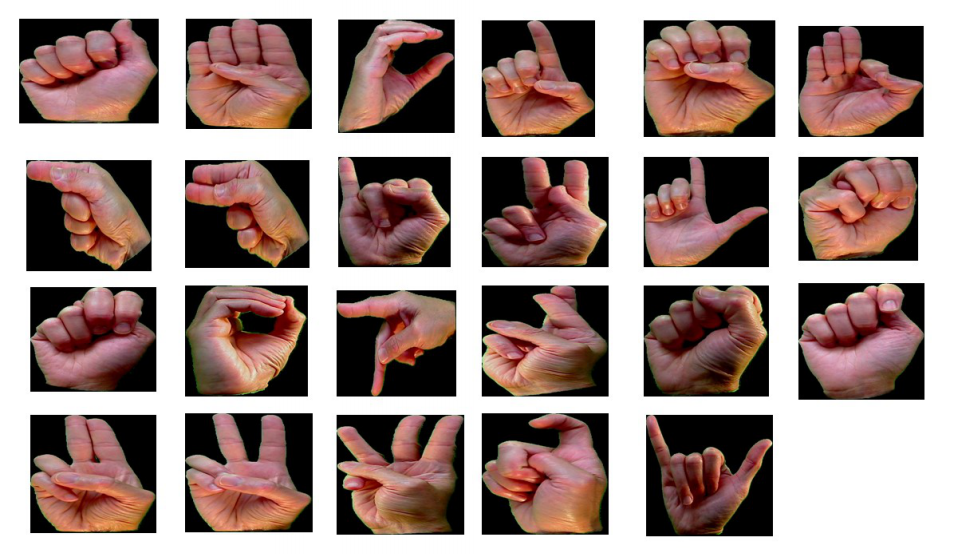
\includegraphics[width=0.8\linewidth]{datasetasl}
	\caption{Sample Dataset ASL Massey University (Barczak et al., 2011)}
	\label{fig:datasetasl}
\end{figure}

Acuan dalam penelitian ini menggunakan dataset angka 0 sampai 9, dengan citra yang sudah di segmentasi.
Dataset ini akan dilatih dalam CNN untuk pengenalan gestur tangan.
Pengambilan dataset \emph{Massey University} dilakukan menggunakan \emph{green screen} sehingga mudah untuk disegmentasi, setup pengambilan dataset dilakukan dengan skema seperti Gambar 4.4 (Barczak et al., 2011).
% TODO: \usepackage{graphicx} required
\begin{figure}[H]
	\centering
	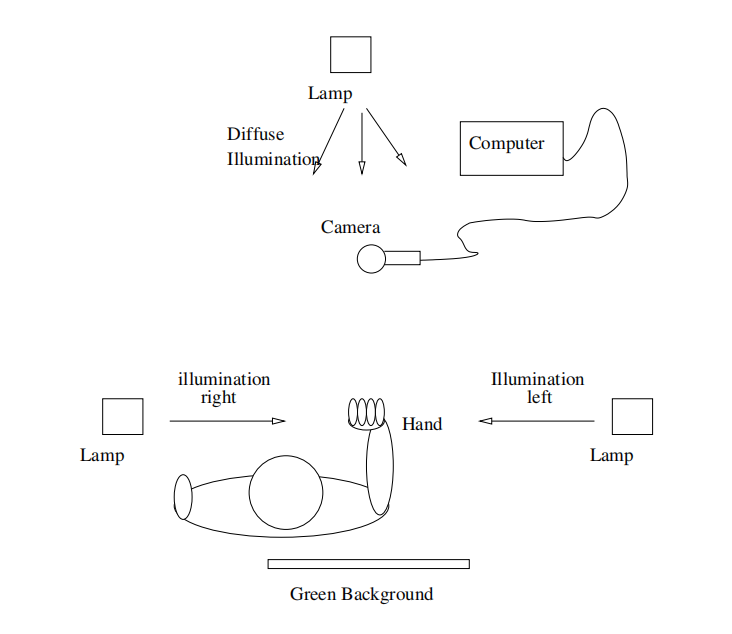
\includegraphics[width=0.8\linewidth]{setup}
	\caption{Setup Pengambilan Dataset (Barczak et al., 2011)}
	\label{fig:setup}
\end{figure}

Pengambilan dataset berikutnya berbeda dengan dataset ASL, dataset berikutnya untuk deteksi tangan tidak memiliki klasifikasi, citra diambil dari 10 orang dengan random pose. 
dataset ini digunakan untuk pelatihan pada object detection. Pengambilan dataset dilakukan masing masing 100 capture untuk setiap orang, 
sehingga pada dataset ini diperoleh 1000 citra.
\section{Proses Pelatihan}
Proses pelatihan dalam penelitian ini dibagi menjadi dua bagian, yaitu pelatihan object detection dan pelatihan gestur recognition.
\subsection{Pelatihan Gesture Recognition}
Dataset pada pelatihan \emph{gesture recognition} menggunakan dataset dari \emph{Massey Univertisy} yang di labeli sesuai acuan ASL dari angka 0 hingga 9. Jumlah dataset adalah 700 citra kemudian dibagi yang akan dibagi dalam \emph{train} dan \emph{test} menggunakan \emph{k-fold cross validation} dengan k = 5.
Proses pelatihan untuk pengenalan gestur tangan menggunakan teknik \emph{transfer learning} yang memiliki kelebihan pada waktu pelatihan dan penggunaan dataset yang cenderung sedikit. \emph{Pre-trained} model yang digunakan adalah \emph{MobileNetV2}. \emph{Pre-trained} model memiliki pengetahuan dari dataset yang telah dilatih sebelumnya, pada \emph{MobileNetV2} telah dilatih menggunakan dataset dari \emph{ImageNet}, kemudian pengetahuan tersebut akan di pindahkan ke model baru dan dilatih sesuai dataset baru, sehingga memiliki keluaran dalam bentuk klasifikasi atau tugas sesuai yang diinginkan.

Masukan citra memiliki dimensi 224x224 piksel yang terdiri 3 channel RGB, sehingga node \emph{input} berjumlah 50176 dengan range 0-255 untuk setiap piksel. Arsitektur jaringan pada pelatihan ini dilakukan dengan mengganti bagian blok klasifikasi dari \emph{MobileNetV2} menjadi klasifikasi dataset ASL. 
Arsitektur transfer learning dapat dilihat pada Gambar 4.5.
% TODO: \usepackage{graphicx} required
\begin{figure}[H]
	\centering
	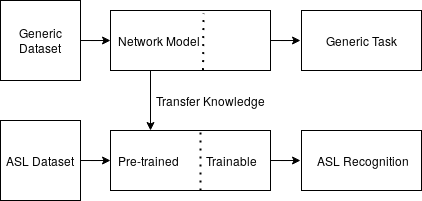
\includegraphics[width=0.8\linewidth]{transfer}
	\caption{Transfer Learning Pelatihan Gestur}
	\label{fig:asritrkturku}
\end{figure}

\subsection{Pelatihan Object Detection}
Proses pelatihan pada \emph{object detection} menggunakan \emph{pre-trained model SSD MobilenetV2 COCO} yang sudah di latih sebelumnya dengan dataset COCO.
Dataset yang baru akan dilatih menggunakan \emph{pre-trained} model, sehingga dengan pengetahuan yang sudah ada dilatih agar menghasilkan model baru sesuai dengan \emph{output} yang diinginkan. 
Dataset yang akan dilatih sejumlah 1000 citra yang telah dilabeli secara manual dengan pembagian 80\% \emph{training} dan 20\% \emph{testing}.
Arsitektur yang digunakan dalam pelatihan \emph{object detection} dapat dilihat pada Gambar 4.6.
\begin{figure}[H]
	\centering
	\includegraphics[width=0.7\linewidth]{"v2"}
	\caption{Arsitektur Mobilenet V2 (Sandler et al., 2018)}
	\label{fig:v2}
\end{figure}
%----------------------------------PENGUJIAN-------------------------------------
\section{Pengujian dan Evaluasi}
Pengujian dan evaluasi adalah tahap untuk mengukur performa dari sebuah sistem. Pengujian ini akan dibagi menjadi 6 tahap, yaitu evaluasi deteksi tangan, evaluasi pengenalan gestur, pengujian deteksi tangan menggunakan \emph{Retinex}, pengujian pengenalan gestur tangan menggunakan \emph{Retinex}, pengujian SNR dan pengujian keseluruhan sistem. 
Setiap pengujian yang menggunakan Retinex dilakukan hal yang sama, yaitu dengan menurunkan intensitas cahaya.
%------------------------------------PENGUJIAN DETEKSI------------------------
\subsection{Evaluasi Deteksi Tangan}
Evaluasi model deteksi tangan dilakukan setelah \emph{training} menggunakan metrik \emph{mean average precicion} (mAP). \emph{Mean average precicion} merupakan metrik yang populer untuk mengevaluasi model dari detektor. \emph{Mean average precicion} merupakan rata rata dari \emph{Average Precicion} (AP) pada setiap nilai IoU. Sesuai dengan acuan COCO dataset untuk mengevaluasi model pada objek detection dengan menghitung mAP dari IoU=0.5 hingga 0.95 dengan pertambahan 0.05.
\subsection{Evaluasi Pengenalan Gestur Tangan}
Evaluasi model CNN untuk pengenalan gestur tangan didapatkan saat \emph{training} dan \emph{testing} menggunakan \emph{k-fold cross validation} dengan k = 5, dimana dilakukan validasi sebanyak 5 kali dengan skenario pengujian yang berbeda pada proses \emph{training} dan \emph{testing}.
\emph{Training accuracy} dan \emph{testing accuracy} didapatkan pada setiap \emph{fold}.
\subsection{Pengujian SNR}
SNR\emph{(Signal to Noise Ratio)} adalah ukuran untuk mengukur kualitas citra terhadap citra yang dilakukan perbaikan. Citra hasil perbaikan dibandingkan dengan citra asli untuk mendapatkan nilai SNR nya. Nilai SNR yang tinggi mengindikasikan kualitas citra yang semakin baik karena rasio sinyal terhadap metode juga tinggi, sebaliknya nilai SNR yang rendah berarti kualitas citra yang di hasilkan semakin buruk atau semakin kecil dalam peningkatan kualitas citra. Pengujian SNR ini dilakukan untuk menentukan nilai dari parameter \emph{retinex} yang akan dipakai pada sistem.
\subsection{Pengujian Deteksi Tangan Menggunakan Retinex}
Tujuan pengujian deteksi tangan dilakukan untuk menguji sistem dalam melakukan deteksi tangan terkait dengan penurunan intensitas cahaya. Skema pengujian deteksi tangan dapat dilihat pada Gambar 4.7.
% TODO: \usepackage{graphicx} required
\begin{figure}[H]
	\centering
	\includegraphics[width=0.19\linewidth]{"skema objek deteksi"}
	\caption{Skema Pengujian Deteksi Tangan}
	\label{fig:skema-objek-deteksi}
\end{figure}
Pada pengujian ini dilakukan secara manual oleh 3 subjek yang berbeda, setiap subjek akan dicatat apakah sistem mampu mendeteksi tangan atau tidak pada intensitas cahaya pada saat itu selama 10 kali, kemudian dilakukan penurunan intensitas sebesar 50\%. Penurunan ini dilakukan hingga sebuah sistem tidak mampu mendeteksi tangan dari subjek. Hasil pengujian akan dicatat dalam bentuk tabel pengujian seperti pada Tabel 4.1. Evaluasi pengujian dilakukan dengan \emph{confussion matrix}, sehingga memperoleh nilai akurasi untuk setiap lux dari hasil pengujian.
\begin{table}[H]
	\caption{Pengujian Deteksi Tangan}
	\vspace{0.2cm}
	\centering
	\begin{tabular}{|c|c|c|c|c|c|c|c|c|c|c|c|c|c|c|c|c|c|c|c|c|c|c|c|c|c|c|c|c|c|c|}
		\hline
		Nilai Lux(X) & \multicolumn{10}{|c|}{Hasil Deteksi Subjek\_1} & \multicolumn{10}{|c|}{Hasil Deteksi Subjek\_2}& \multicolumn{10}{|c|}{Hasil Deteksi Subjek\_3}\\
		\hline X & & & &&&&&&&&&&&&&&&&&&&&&&&&&&&\\
		\hline X=X*50\% & & & &&&&&&&&&&&&&&&&&&&&&&&&&&&\\
		\hline X=X*50\% & & & & && &&&&&&&&&&&&&&&&&&&&&&&&\\
		\hline X=X*50\% & & & &&&&&&& &&&&&&&&&&&&&&&&&&&&\\
		\hline $\dots$ & & & & & &&&&&&&&&&&&&&&&&&&&&&&&&\\
		\hline X=X $\le$ 50Lux & & & &&&&&&& &&&&&&&&&&&&&&&&&&&&\\
		\hline
	\end{tabular}
\end{table}
%------------------------------PENGUJIAN GESTUR------------------------------------
\subsection{Pengujian Pengenalan Gestur Tangan Menggunakan Retinex}
Pengujian tahap kedua yaitu pengenalan gestur tangan dengan \emph{retinex}. Tujuan dari pengujian ini untuk mengukur performa sistem dalam melakukan pengenalan gestur tangan dengan acuan ASL sesuai dengan dataset yang telah dilatih. Skema pengujian pengenalan gestur tangan dapat dilihat pada Gambar 4.8.
% TODO: \usepackage{graphicx} required
\begin{figure}[H]
	\centering
	\includegraphics[width=0.19\linewidth]{"proses pengujian sistem"}
	\caption{Skema Pengujian Pengenalan Gestur Tangan}
	\label{fig:screenshot-from-2020-03-04-22-24-45}
\end{figure}
Pengujian pengenalan dilakukan secara manual dan terpisah dari deteksi objek, tahap ini memiliki perlakuan sama dengan tahap sebelumnya, yaitu menggunakan 3 subjek yang berbeda, kemudian dilakukan pengenalan gestur tangan sebanyak 10 kali untuk setiap klasifikasi. Total citra yang didapat dalam satu kondisi lux oleh satu subjek adalah 100 citra.
Tahap berikutnya dilakukan penurunan intensitas cahaya, dengan mengatur cahaya lampu di ruangan uji sebesar 50\% lux menggunakan dimmer. Pengujian dilakukan hingga batas lux kurang dari 50 lux.
\begin{table}[H]
	\caption{Pengujian Pengenalan Gestur Tangan}
	\vspace{0.2cm}
	\centering
\begin{tabular}{|c|}
	\hline
	\multicolumn{1}{|c|}{Nilai Lux(X)}\\

	\begin{tabular}{|c|c|c|c|c|c|c|c|c|c|c|c|c|c|c|c|c|c|c|c|c|c|c|c|c|c|c|c|c|c|c|c|c|}
		\hline
		Klasifikasi & \multicolumn{10}{|c|}{Pengenalan Subjek\_1}& \multicolumn{10}{|c|}{Pengenalan Subjek\_2}& \multicolumn{10}{|c|}{Pengenalan Subjek\_3}\\
		\hline Angka 0 & & & &&&&&&&&&&&&&&&&&&&&&&&&&&&\\
		\hline Angka 1 & & & &&&&&&&&&&&&&&&&&&&&&&&&&&&\\
		\hline Angka 2 & & & & && &&&&&&&&&&&&&&&&&&&&&&&&\\
		
		\hline ... & & & &&&&&&&&&&&&&&&&&&&&&&&&&&& \\
		\hline Angka 9 & & & &&&&&&&&&&&&&&&&&&&&&&&&&&& \\
		\hline
	\end{tabular}
\end{tabular}
%%======================================================
\begin{tabular}{|c|}
	\multicolumn{1}{|c|}{Nilai Lux(...)}\\	
	\begin{tabular}{|c|c|c|c|c|c|c|c|c|c|c|c|c|c|c|c|c|c|c|c|c|c|c|c|c|c|c|c|c|c|c|c|c|}
		\hline
		Klasifikasi & \multicolumn{10}{|c|}{Pengenalan Subjek\_1}& \multicolumn{10}{|c|}{Pengenalan Subjek\_2}& \multicolumn{10}{|c|}{Pengenalan Subjek\_3}\\
		\hline Angka 0 & & & &&&&&&&&&&&&&&&&&&&&&&&&&&&\\
		\hline Angka 1 & & & &&&&&&&&&&&&&&&&&&&&&&&&&&&\\	
		\hline Angka 2 & & & &&&&&&&&&&&&&&&&&&&&&&&&&&&\\	
		\hline ... & & & &&&&&&&&&&&&&&&&&&&&&&&&&&& \\
		\hline Angka 9 & & & &&&&&&&&&&&&&&&&&&&&&&&&&&& \\
		\hline
	\end{tabular}	
\end{tabular}
%%======================================================
\begin{tabular}{|c|}

	\multicolumn{1}{|c|}{Nilai Lux(X$\le$50)}\\
	\begin{tabular}{|c|c|c|c|c|c|c|c|c|c|c|c|c|c|c|c|c|c|c|c|c|c|c|c|c|c|c|c|c|c|c|c|c|}
		\hline
		Klasifikasi & \multicolumn{10}{|c|}{Pengenalan Subjek\_1}& \multicolumn{10}{|c|}{Pengenalan Subjek\_2}& \multicolumn{10}{|c|}{Pengenalan Subjek\_3}\\
		\hline Angka 0 & & & &&&&&&&&&&&&&&&&&&&&&&&&&&&\\
		\hline Angka 1 & & & &&&&&&&&&&&&&&&&&&&&&&&&&&&\\	
		\hline Angka 2 & & & &&&&&&&&&&&&&&&&&&&&&&&&&&&\\
		\hline ... & & & &&&&&&&&&&&&&&&&&&&&&&&&&&& \\
		\hline Angka 9 & & & &&&&&&&&&&&&&&&&&&&&&&&&&&& \\
		\hline
	\end{tabular}
\end{tabular}

\end{table}

Hasil dari pengujian akan di catat dalam bentuk tabel seperti pada Tabel 4.2. Evaluasi pengujian dilakukan dengan \emph{confussion matrix}, sehingga memperoleh nilai akurasi dari hasil pengujian. Perhitungan akurasi dilakukan pada setiap nilai lux yang di uji.
\subsection{Pengujian Sistem Keseluruhan}
Pengujian tahap terakhir adalah pengujian keseluruhan sistem yang dilakukan secara manual, dengan menggabungkan \emph{retinex}, deteksi objek dan pengenalan gestur tangan dalam satu program utuh. Pengenalan akan terjadi apabila sebuah tangan dideteksi terlebih dahulu, jika tidak terdeteksi maka tidak akan dilakukan pengenalan. Penurunan intensitas dilakukan sama seperti pengujian sebelumnya. Tabel pengujian yang digunakan mengacu pada Tabel 4.2. Evaluasi dari akurasi sistem keseluruhan dapat diperoleh menggunakan \emph{confusion matrix}.